\documentclass[11pt,a4paper]{article}
\usepackage[margin=2cm]{geometry}
\usepackage[T1]{fontenc}
\usepackage{mathptmx}
\usepackage{amsmath,amssymb}
\usepackage{graphicx}
\usepackage{xcolor}
\usepackage{enumitem}
\usepackage{array}
\usepackage{float}
\usepackage[hidelinks]{hyperref}
\graphicspath{{figs/}}
\definecolor{navy}{HTML}{1B3755}
\setlength{\parindent}{0pt}
\setlength{\parskip}{5pt}
\renewcommand{\arraystretch}{1.22}
\newcommand{\sect}[1]{\bigskip{\Large\color{navy}\bfseries #1}\par\smallskip{\color{navy}\hrule height 0.8pt}\smallskip}
\newcommand{\sub}[1]{\medskip{\large\color{navy}\bfseries #1}\par}
\newcommand{\say}[1]{\par\smallskip\noindent\fbox{\parbox{\dimexpr\linewidth-2\fboxsep-2\fboxrule}{\textbf{In one sentence:} #1}}\par}

\begin{document}
\begin{center}
{\LARGE\bfseries\color{navy} How DG Degrades the CTI, and How the DSDR Mitigates It}\\[4pt]
{\large A complete guide with the results of the study}\\[2pt]
IEEE 13-node feeder, DIgSILENT PowerFactory --- Jhala Nath Kafle (081MSPSE009)
\end{center}

\sect{1. The quantity: coordination time interval (CTI)}
For fuse saving the recloser must open on its fast curve \emph{before} the fuse starts to melt:
\[
\mathrm{CTI} = t_{MMT}(I_{fuse}) - t_{fast}(I_{rec})
\]
\begin{itemize}[leftmargin=*,itemsep=2pt]
\item $t_{MMT}$: minimum melting time of the fuse at the current through the fuse.
\item $t_{fast}$: fast operating time of the recloser at the current through the recloser.
\item CTI $>0$: the recloser wins, the fuse is saved. CTI $<0$: the fuse melts first, fuse saving is lost.
\end{itemize}
Without DG the fuse and the recloser are in series and carry the \emph{same} current, so the CTI is fixed by the
shape of the two curves. With DG this is no longer true --- that is the whole problem.

\sect{2. How the study measured it}
\begin{itemize}[leftmargin=*,itemsep=2pt]
\item Seven PowerFactory models, DG at node 692 at 0, 10, 25, 37, 50, 75 and 100\,\% of 4.05\,MVA. The main model
  was not changed.
\item Two faults, as in the reference method:
  \textbf{internal fault at 633} (bolted LLL; fuse F633 against R1) --- the DG is \emph{beyond} the recloser, between
  the fault and R2;
  \textbf{external fault at 684} (fuse F671-2 against R2) --- the DG is on the same side as the fault, downstream
  of R2.
\item Two protection schemes: \textbf{conventional} (single-setting R2, fuses of the design without DG, F633 250E)
  and \textbf{DSDR} (R2 with forward and reverse groups designed for 100\,\% DG, revised fuses, F633 400E).
\item All times are PowerFactory's own relay and fuse times.
\end{itemize}

\sect{3. How DG degrades the CTI}
\sub{3.1 The mechanism in three steps}
\begin{enumerate}[leftmargin=*,itemsep=3pt]
\item \textbf{The fuse sees more current.} For a fault at 633 the fuse F633 lies between the fault and \emph{both}
  sources. It carries the grid current \emph{plus} the DG current:
  $I_{fuse} = I_{grid} + I_{DG}$.
\item \textbf{The recloser sees the same or less.} R1 carries only the grid share. The DG even holds the network
  voltage up during the fault, so the grid share \emph{falls} slightly as the DG grows.
\item \textbf{The fuse curve is steep.} A fuse follows roughly $t \propto I^{a}$ with $a \approx -1.8$
  (eq.~9 of the method), much steeper than the recloser curve in this range. A small rise of the fuse current
  shortens its melting time a lot, while the small fall of the recloser current lengthens its time only a little.
  The CTI shrinks and changes sign.
\end{enumerate}

\textbf{Check with the numbers (0 $\rightarrow$ 100\,\%, fault at 633):} the fuse current rises by a factor
$5426/4102 = 1.32$, so $t_{MMT}$ should fall by about $1.32^{-1.8} = 0.61$; PowerFactory gives
$0.0548/0.1018 = 0.54$. The R1 current falls from 4162 to 3970\,A (-4.6\,\%) and its fast time rises only from
0.098 to 0.106\,s (+8\,\%).

\sub{3.2 Internal fault at 633, conventional protection}
\begin{center}\small
\begin{tabular}{|c|c|c|c|c|c|c|}
\hline
\textbf{DG} & \textbf{DG (MVA)} & \textbf{$I_{F633}$ (A)} & \textbf{$I_{R1}$ (A)} & \textbf{$t_{MMT}$ F633 (s)} &
\textbf{$t_{fast}$ R1 (s)} & \textbf{CTI (ms)} \\ \hline
0\,\% & 0.00 & 4102 & 4162 & 0.102 & 0.098 & $+4$ \\ \hline
10\,\% & 0.41 & 4256 & 4142 & 0.094 & 0.099 & $-5$ \\ \hline
25\,\% & 1.01 & 4478 & 4111 & 0.083 & 0.100 & $-17$ \\ \hline
37\,\% & 1.50 & 4648 & 4088 & 0.077 & 0.101 & $-24$ \\ \hline
50\,\% & 2.02 & 4824 & 4062 & 0.071 & 0.102 & $-31$ \\ \hline
75\,\% & 3.04 & 5140 & 4015 & 0.062 & 0.104 & $-42$ \\ \hline
100\,\% & 4.05 & 5426 & 3970 & 0.055 & 0.106 & $-51$ \\ \hline
\end{tabular}
\end{center}
The margin without DG was only +4\,ms, so the CTI turns negative at about 4\,\% penetration.

\sub{3.3 External fault at 684, conventional protection}
\begin{center}\small
\begin{tabular}{|c|c|c|c|c|c|}
\hline
\textbf{DG} & \textbf{$I_{F671\text{-}2}$ (A)} & \textbf{$I_{R2}$ (A)} & \textbf{$t_{MMT}$ F671-2 (s)} &
\textbf{$t_{fast}$ R2 (s)} & \textbf{CTI (ms)} \\ \hline
0\,\% & 2574 & 2711 & 0.470 & 0.067 & $+403$ \\ \hline
25\,\% & 2926 & 2636 & 0.323 & 0.069 & $+254$ \\ \hline
50\,\% & 3276 & 2557 & 0.237 & 0.072 & $+166$ \\ \hline
75\,\% & 3623 & 2511 & 0.184 & 0.073 & $+110$ \\ \hline
100\,\% & 3963 & 2543 & 0.148 & 0.072 & $+75$ \\ \hline
\end{tabular}
\end{center}
Same mechanism (the DG at 692 feeds the fault at 684 through F671-2 but not through R2). The CTI falls by
81\,\% but stays positive, because the margin without DG was large.

\begin{figure}[H]\centering
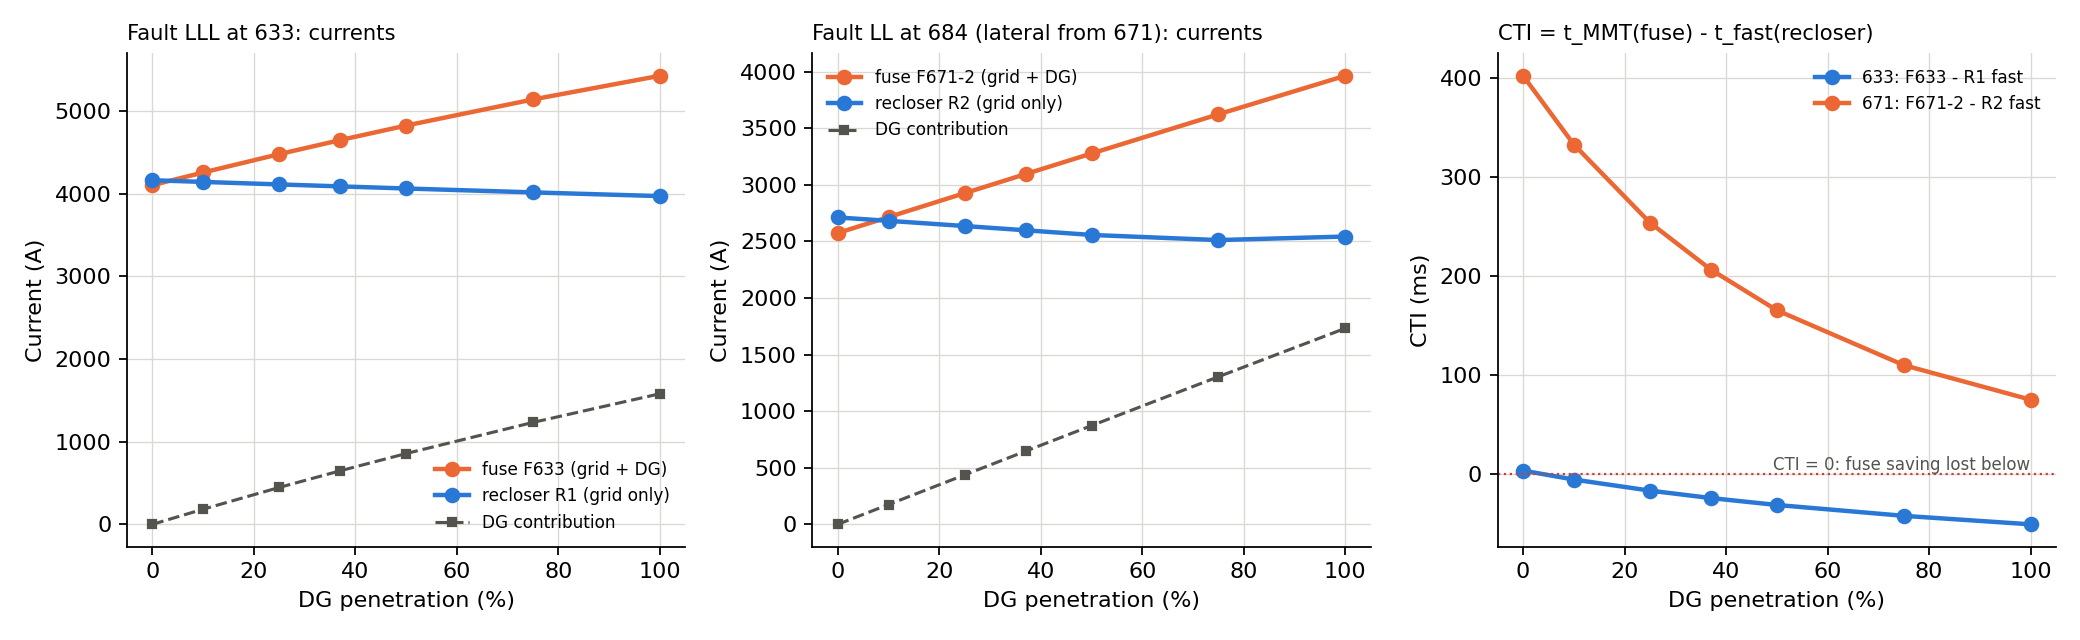
\includegraphics[width=0.95\textwidth]{pen_currents.png}
\caption*{\small Fuse current (grid + DG), recloser current (grid only), DG current and resulting CTI against DG penetration.}
\end{figure}

\sub{3.4 The other effects of rising penetration}
\begin{itemize}[leftmargin=*,itemsep=3pt]
\item \textbf{Fault level rises}, most near the DG: 671/692 +64\,\%, 675 +59\,\%, 684 +55\,\%, 633 +32\,\%,
  632 +38\,\%. Least behind the transformer (634, +12\,\%) and on the single-phase laterals (+19--20\,\%).
\item \textbf{Reverse current through R2} for faults upstream of it grows: fault at 633, 66\,A at 0\,\% to
  1500\,A at 100\,\%. A conventional (non-directional) R2 starts to trip on it from about 37\,\% --- a trip for a
  fault outside its zone, which also disconnects the healthy part beyond 671 together with the DG.
\item \textbf{Load flow reverses.} The power through R2 falls from 2460\,kW towards 671 (0\,\%) to 755\,kW
  towards 632 (100\,\%); the current through R1 falls from 588 to 285\,A.
\item \textbf{Loss of sensitivity.} The weakest fault in R2's zone (LG through 3\,$\Omega$) falls from 879\,A to
  368\,A, below R2's 600\,A start from about 75\,\%: R2 no longer sees it.
\end{itemize}

\say{The fuse carries grid plus DG current while the recloser carries only the grid share; because the fuse
curve is much steeper, the fuse becomes faster far more quickly than the recloser, and the CTI falls with every
step of DG penetration.}

\sect{4. How the DSDR mitigates it}
\sub{4.1 Two actions that work together}
\begin{enumerate}[leftmargin=*,itemsep=3pt]
\item \textbf{A reverse setting group on R2.} For a fault at 633 the DG current flows backwards through R2. A
  conventional R2 is set for the large forward grid current and is slow or blind to this smaller current. The
  reverse group has a lower pickup (150/300\,A plugs, curve from 300\,A) and trips fast on it: at 100\,\% DG
  R2 reverse fast = 0.060\,s (conventional R2: 0.160\,s). R1 removes the grid share, R2 removes the DG share, so
  \emph{both} sources are cut before the fuse melts.
\item \textbf{The fuse revision.} The fuse is made one or two sizes larger (F633 250E $\rightarrow$ 400E), so its
  melting curve moves up and the margin over R1 is restored. This is allowed only because the dial ranges were
  exhausted (step 9 of the method). The revision alone is not enough: with revised fuses but a conventional R2
  only 31 of 39 cells are held; with the DSDR, 38.
\end{enumerate}

\sub{4.2 Internal fault at 633: conventional against DSDR}
\begin{center}\small
\begin{tabular}{|c|c|c|c|c|c|}
\hline
 & \multicolumn{2}{c|}{\textbf{CTI against R1 (ms)}} & \multicolumn{2}{c|}{\textbf{R2 fast trip (s)}} & \\
\textbf{DG} & \textbf{Conventional} & \textbf{DSDR} & \textbf{Conventional} & \textbf{DSDR reverse} &
\textbf{DSDR margin to last fast trip (ms)} \\ \hline
0\,\% & $+4$ & $+205$ & no trip & no trip & $+205$ \\ \hline
10\,\% & $-5$ & $+175$ & no trip & no trip & $+175$ \\ \hline
25\,\% & $-17$ & $+139$ & no trip & 0.518 & $-279$ \\ \hline
37\,\% & $-24$ & $+116$ & 1.109 & 0.231 & $-14$ \\ \hline
50\,\% & $-31$ & $+96$ & 0.551 & 0.140 & $+57$ \\ \hline
75\,\% & $-42$ & $+65$ & 0.250 & 0.080 & $+65$ \\ \hline
100\,\% & $-51$ & $+43$ & 0.160 & 0.060 & $+43$ \\ \hline
\end{tabular}
\end{center}
\begin{itemize}[leftmargin=*,itemsep=3pt]
\item \textbf{CTI against R1 stays positive at every level} with the DSDR (+205 $\rightarrow$ +43\,ms) instead of
  turning negative (+4 $\rightarrow$ -51\,ms). The DG still erodes it (by 162\,ms), but from a much larger start.
\item \textbf{Margin to the last fast trip} (fuse melting time minus the later of R1's and R2's fast trips --- the
  strict test, because the DG current keeps heating the fuse until R2 opens): positive at 0--10\,\% (the DG current
  is too small to matter) and from 50\,\% up. At 0--10\,\% the DG current through F633 (66--161\,A) is below the
  fuse's melting range, so the fuse survives even though R2 does not trip.
\item \textbf{The weak spot at 25--37\,\%.} The reverse group was designed for 100\,\% DG. At low penetration the DG
  current (416--610\,A) is only just above its 300\,A start, so the reverse fast trip is slow (0.518 and 0.231\,s)
  and the margin is negative ($-279$ and $-14$\,ms). The conventional R2 is worse there: it does not trip at 25\,\%
  and trips only after 1.109\,s at 37\,\% ($-1033$\,ms). The remedy is adaptive: a reverse group selected for the
  actual DG output --- listed as future work.
\end{itemize}

\begin{figure}[H]\centering
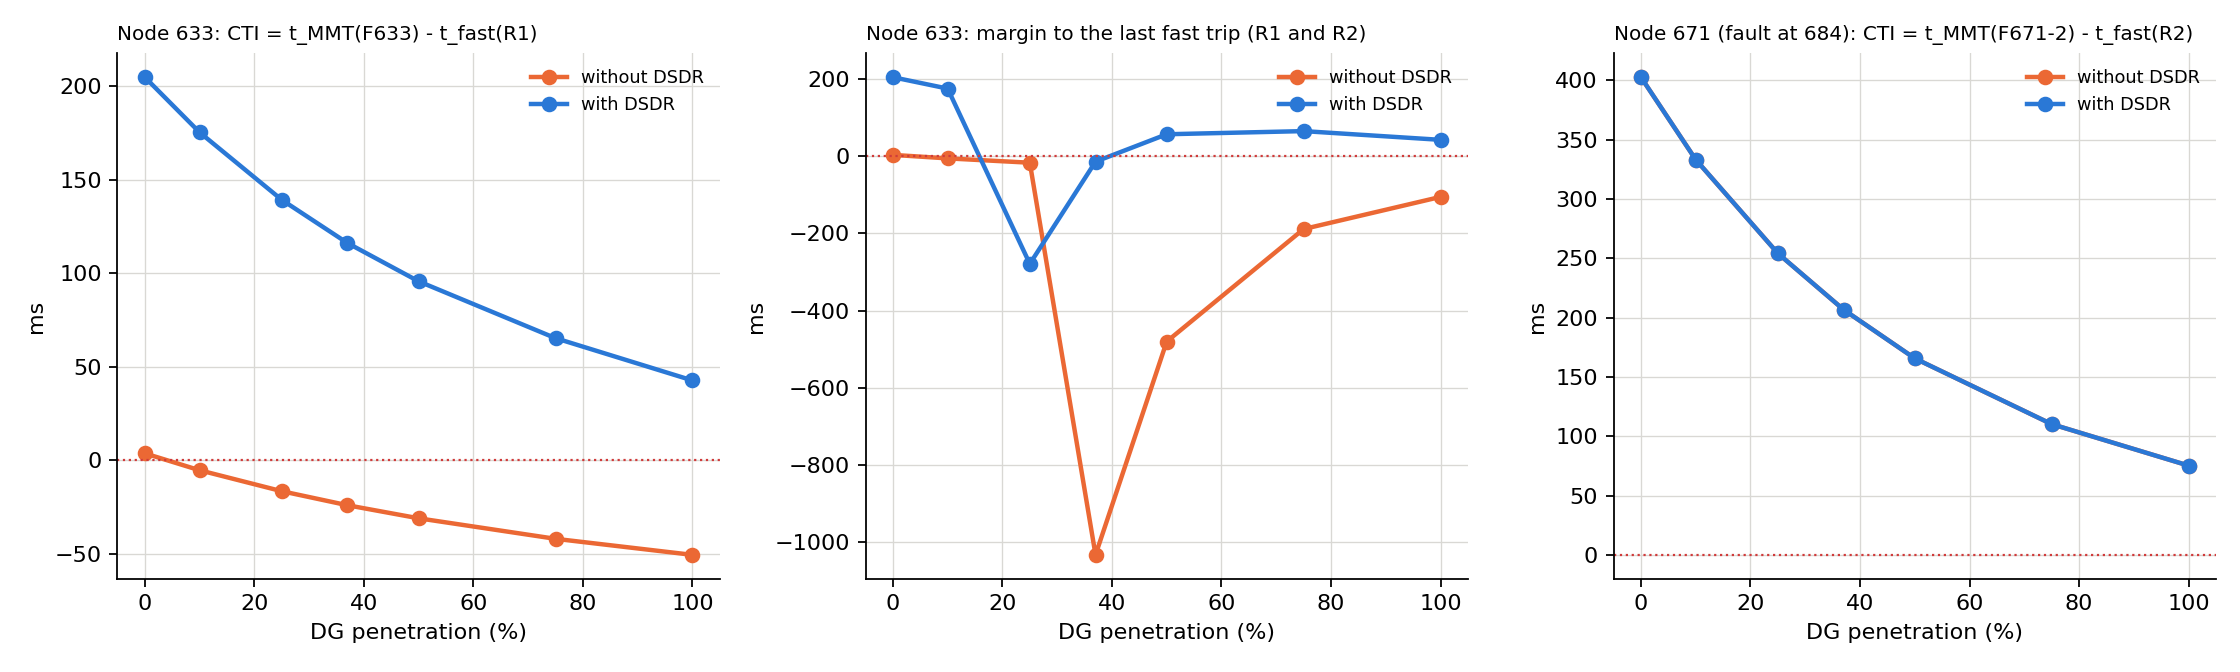
\includegraphics[width=\textwidth]{CTI_conventional_vs_DSDR.png}
\caption*{\small Left: CTI at 633 against R1. Middle: margin to the last fast trip at 633 (R1 and R2). Right: CTI
for the fault at 684 --- identical for both schemes.}
\end{figure}

\sub{4.3 External fault at 684: the DSDR does not help}
The CTI at 671 is identical in both schemes (+403 $\rightarrow$ +75\,ms). For a fault downstream of R2 the current
through R2 is forward, so the forward group is used, which is the same in both schemes, and F671-2 is not
revised. The DG at 692 feeds this fault directly, with no recloser in its path, so no setting of R2 can remove the
DG share. This is a limit of the DSDR concept itself; it is also why the time-sequence check shows ``DG keeps
feeding'' for all 21 cells below R2.

\sub{4.4 The same effect in the full coordination study (DG 4.05\,MVA)}
\begin{center}\small
\begin{tabular}{|l|c|}
\hline
\textbf{Protection} & \textbf{Cells held (of 39)} \\ \hline
No DG, design fuses & 39 \\ \hline
DG, conventional R2, design fuses & 24 \\ \hline
DG, DSDR, design fuses & 25 \\ \hline
DG, conventional R2, revised fuses & 31 \\ \hline
DG, DSDR, revised fuses & \textbf{38} \\ \hline
\end{tabular}
\end{center}
Example (three-phase fault near 632, R2 carries 1777\,A in reverse): single setting, R2 fast 0.121\,s and F633
melts at 0.100\,s --- lost; dual setting, R2 reverse fast 0.052\,s --- held.

\say{The DSDR gives R2 a reverse group that cuts the DG's share of the fault current quickly, and the fuse revision
restores the fuse's head-start over R1; together they keep the CTI positive for faults between the grid and the
DG, but they cannot help faults downstream of R2, where the DG feeds the fault directly.}

\sect{5. Likely questions}
\textbf{Why does the CTI decrease and not increase?} Because the fuse sees grid + DG and the recloser only grid; the
fuse becomes relatively faster. If the recloser carried the larger current (fault upstream of the fuse's source
side), the opposite would happen, but in this topology the fuse is always the device nearer the fault.

\textbf{Does the DSDR stop the CTI from falling?} No. It keeps it positive. The DG still erodes the margin
(633: $-162$\,ms from 0 to 100\,\%), but the DSDR and the fuse revision start from a much larger margin and the
reverse group removes the DG current.

\textbf{Why is the DSDR worse than conventional at 25\,\% in the margin column?} It is not worse in practice: the
conventional R2 never trips there, so the margin column ignores it, while the slow reverse trip of the DSDR (0.518\,s)
is counted. The column is a strict, conservative measure. The real cure is a reverse group adapted to the DG output.

\textbf{What would you do for faults below R2?} The DG must be disconnected or a recloser/protection placed at the DG
connection, or the fuses below R2 sized for grid + DG current; the DSDR alone cannot solve it.
\end{document}
